\chapter{ابزار هدف}
خصیصه‌های مطرح در مدل کیفیتی انتخاب شده، به طور خاص بیان‌گر نحوه اندازه‌گیری نیستند و می‌بایست به منظور رسیدن به یک ابزار درست، در ابتدا مدل‌ کیفیتی انتخاب شده را کمی شفاف‌تر کنیم تا نیازمندی‌ها به صورت دقیق‌تر مشخص شوند. به همین منظور می‌بایست تمامی یازده خصیصه کیفیتی مرتبط با استفاده‌پذیری را به تفصیل شرح داده و روش‌های اتخاذی خود را برای اندازه‌گیری هرکدام مطرح کنیم. از آن‌جا که هدف این پروژه تولید یک نرم‌افزار است، می‌بایست در قدم بعدی به بیان نمودارهای مرتبط بپردازیم و پس از پیاده‌سازی آزمایش‌های لازم را انجام داده و نتایج را ذکر کنیم. در طول این فصل به موارد ذکر شده پرداخته‌ایم که به ترتیب مورد بحث واقع شده‌اند.
\section{کشف نیازمندی‌ها}
ابزار مورد نظر می‌بایست قابلیت اندازه‌گیری استفاده‌پذیری در ذیل مدل کیفیتی مطرح شده در فصل پیشین (مدل تولیس
\cite{albert_measuring_2013})
را داشته باشد. بنابراین توجه به خصیصه‌های کیفیتی مطرح شده در این مدل، اولویت شماره اول است. بررسی مدل‌های کیفیتی مختلف (رجوع شود به جدول
\ref{tab:models})
بیانگر این است که در تبیین مدل‌های کیفیتی به دلیل کل‌نگر بودن و پرهیز از انحصاری شدن، می‌بایست تا حد امکان از بیان جزییات خصیصه‌ها خودداری کرد؛ اما در ساخت ابزارهای تست و سنجش کیفیت، بدون داشتن جزییات کافی از نحوه اندازه‌گیری، نخواهیم توانست که به سرمنزل مقصود برسیم. بنابراین می‌توان گفت که مهم‌ترین رسالت این پروژه، پر کردن خلا بین نیازمندی‌های نرم‌افزاری و مدل کیفیتی اتخاذ شده است.
\subsection{تجمیع نتایج پیشین و جمع‌بندی}
\begin{table}[H]
	\caption[
	تجمیع نتایج بررسی بهترین روش‌ها و ابزارها
	]{
		تجمیع نتایج بررسی بهترین روش‌ها و ابزارها؛ مطابق این تجمیع، مشاهده می‌شود که در ابزارها و روش‌ها و تکنیک‌های مطالعه استفاده‌پذیری، هشت الگوی تکراری، به منظور انجام ده سناریوی مهم در مطالعه استفاده‌پذیری استفاده شده‌اند.
	}
	\label{tab:tools_aggregated}
	\centering
	\begin{tabular}{|c|c|}
		\hline
		روش سنجش و اندازه‌گیری & دفعات تکرار الگو \\ \hline
		استفاده از حسگر ردیاب چشم & 4 \\ \hline
		بررسی فنی کد صفحات & 9 \\ \hline
		تست‌های مرتبط با حافظه کوتاه‌مدت & 18 \\ \hline
		تست پیمایشی & 24 \\ \hline
		پرسش سوالات مربوط به طرح‌های مفهومی & 30 \\ \hline
		تست ترجیح & 46 \\ \hline
		ذخیره‌سازی کلیک‌های کاربران و پروفایل‌سازی & 56 \\ \hline
		پرسشنامه متنی و تصویری & 59 \\ \hline
	\end{tabular}
\end{table}
با توجه به جدول
\ref{tab:scenario_measurement}
و همچنین نتایج ذکر شده در انتهای فصل پیشین، می‌توان به منظور درک اهمیت هرکدام از الگوها، مطالعه دیگری انجام داد؛ بد نیست به تجمیع داده‌های موجود در این جدول بیندیشیم. در این صورت به نتیجه بسیار جالب ذکر شده در جدول
\ref{tab:tools_aggregated}
خواهیم رسید که شکل
\ref{fig:tools_aggregation}
نیز بیانگر چهره دیگری از این جدول می‌باشد؛ بر اساس اطلاعات موجود در این شکل، ملاحظه می‌شود که دو الگوی بررسی فنی کد و استفاده از ردیاب، در تعداد کمی از مطالعات مورد استفاده قرار گرفته‌اند. در عمل، این دو الگو به خاطر بررسی مواردی خاص در نظر گرفته شده‌اند که در این موارد به منظور رسیدن به نتیجه‌ای مطلوب، می‌بایست از این‌چنین جزئیاتی نیز اطلاع داشته باشیم. اما نباید از این نکته غافل شد که این دو الگو نیازمند صرف وقت و هزینه بسیار زیادی می‌باشند؛ بدیهی است که برای ثبت داده‌های مربوط به نقطه تمرکز چشم کاربر، نیازمند شرایط، تجهیزات و فضای آزمایشگاهی خاص و گران قیمت خواهیم بود. همچنین به منظور بررسی دقیق و موشکافانه کد تولید شده نهایی، می‌بایست زمان زیادی را در ابتدا برای تولید ابزار طی کنیم که مطلوب ما نیست و می‌ةوان از سرویس‌هایی آماده و رایگانی همچون
\lr{Google Lighthouse}
استفاده کرد.
\begin{figure}[H]
	\centering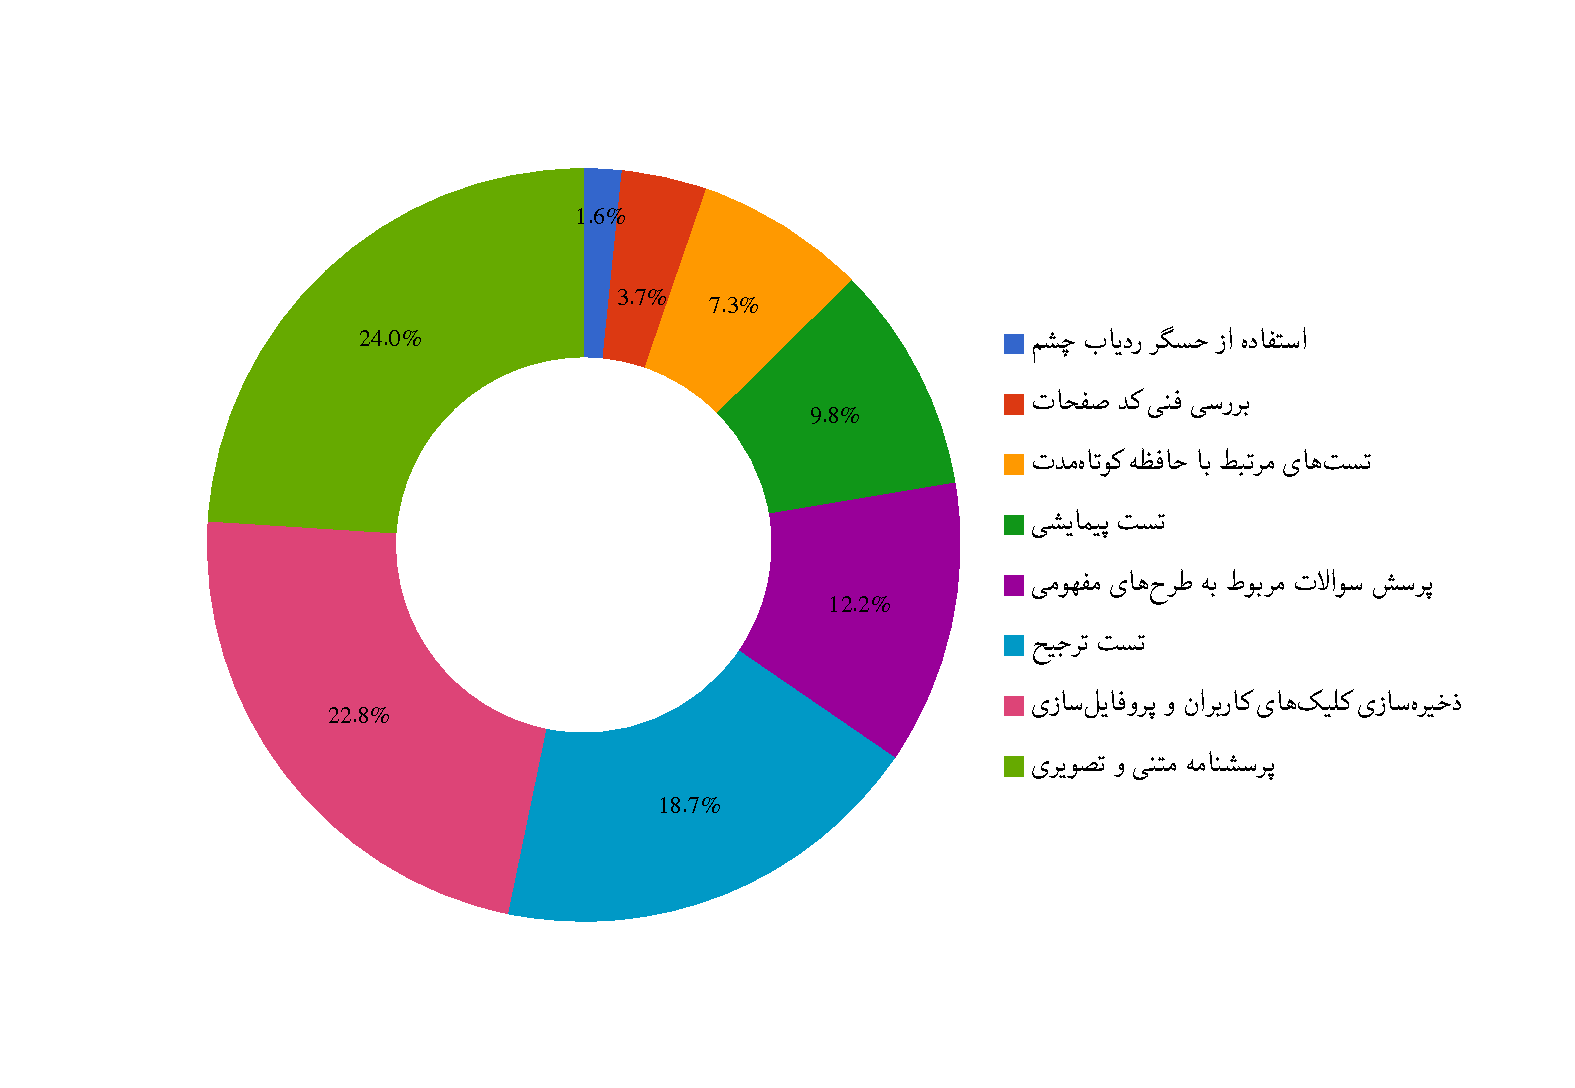
\includegraphics[width=\linewidth]{Resources/percentage.PNG}
	\caption[درصد فراوانی تکرار هر الگو در ابزارهای مورد بررسی]
	{درصد فراوانی تکرار هر الگو در ابزارهای مورد بررسی؛ مشاهده می‌شود که الگوهای ردیابی چشم و همچنین بررسی فنی کد، به دفعات کمتری مورد استفاده قرار گرفته‌اند چرا که کاربر بسیار محدود و جزئی‌ای در مطالعه استفاده‌پذیری دارند. در مقابل اما پرسشنامه‌ها و روش‌های پروفایل‌سازی بیشتر مطرح بوده‌اند.
	}
	\label{fig:tools_aggregation}
\end{figure}
\subsection{مهندسی نیازمندی‌ها}
حال به منظور مرور خصیصه‌های استفاده‌پذیری  و همچنین سناریوهای مطالعه استفاده‌پذیری و نیز اختصاص دادن یک شماره به هرکدام، در ادامه مجددا آن‌ها را یادآوری می‌کنیم؛ مطابق جدول
\ref{tab:10usability}،
سناریو‌های مطالعه استفاده‌پذیری و خصیصه‌های مورد توجه در هر کدام عبارتند از:
\begin{enumerate}
	\item
	انجام یک تراکنش: در این سناریو، خصیصه‌های «موفقیت آمیز بودن وظیفه»، «بهره‌وری کاربر»، «خصیصه‌های موردی»، «خصیصه‌های خود اعلامی» و همچنین «خصیصه‌های وبسایت بلادرنگ» می‌توانند مورد اندازه‌گیری و سنجش قرار می‌گیرند.
	\item
	مقایسه محصولات: با انجام این سناریو، می‌توان خصیصه‌های «موفقیت‌آمیز بودن وظیفه»، «بهره‌وری کاربر»، «خصیصه‌های خوداعلامی» و همچنین «خصیصه‌های ترکیبی و مقایسه‌ای» را مورد بررسی، سنجش و اندازه‌گیری قرار داد.
	\item
	ارزیابی استفاده مکرر از محصول: که در صورت انجام، «موفقیت‌آمیز بودن وظیفه»، «زمان انجام وظیفه»، «بهره‌وری»، «یادگیری‌پذیری» و نیز «خصیصه‌های خود اعلامی» را می‌توان مورد سنجش قرار داد.
	\item
	ارزیابی پیمایش و معماری اطلاعات سامانه: با اجرای این سناریو می‌توان «موفقیت‌آمیز بودن وظیفه»، «خطاها»، «بهره‌وری کاربر» و همچنین «الگوهای مرتب‌سازی» را مورد سنجش و ارزیابی قرار داد.
	\item
	افزایش آگاهی: با انجام مطالعه استفاده‌پذیری به منظور رسیدن به این هدف، می‌توان «خصیصه‌های خوداعلامی»، «خصیصه‌های فیزیولوژیکی و رفتاری» و همچنین «خصیصه‌های وبسایت‌ بلادرنگ» را مورد بحث و بررسی قرار داد.
	\item
	کشف مشکل: با در نظر قرار دادن این سناریو در انجام مطالعات استفاده‌پذیری، می‌توان «خصیصه‌های موردی» و «خصیصه‌های خوداعلامی» را مورد سنجش و ارزیابی قرار داد.
	\item 
	حداکثرسازی استفاده‌پذیری یک محصول حیاتی: هنگامی که این هدف مدنظر باشد، می‌توان «موفقیت‌آمیز بودن وظیفه»، «خطاها» و «بهره‌وری کاربر» را مورد توجه، سنجش و ارزیابی قرار داد.
	\item 
	ایجاد تجربه کاربری مثبت:
	در مطالعه استفاده‌پذیری به منظور ایجاد تجربه کاربری مثبت، «خصیصه‌های خوداعلامی» و همچنین «خصیصه‌های فیزیولوژیکی و رفتاری» که جزوی از ویژگی‌های کاربر نیز هستند، می‌توانند مورد توجه، ارزیابی و سنجش قرار بگیرند.
	\item 
	ارزیابی تاثیرات تغییرهای جزئی و نامحسوس: اگر مطالعه‌ای با این هدف انجام بگیرد، می‌تواند خصیصه‌ای همچون «خصیصه‌های وبسایت بلادرنگ» را با جزئیات زیادی مورد توجه خود واقع کند و به سنجش آن‌ها بپردازد.
	\item
	مقایسه طراحی‌های مختلف: که بیشتر به منظور بیشینه کردن راحتی کاربران هستند، می‌توانند برای سنجش و ارزیابی «موفقیت‌آمیز بودن وظیفه»‌، «زمان انجام وظیفه»، «خصیصه‌های موردی»، «خصیصه‌های خوداعلامی» و همچنین «خصیصه‌های ترکیبی و مقایسه‌ای» به کار گرفته شوند.
\end{enumerate}
\begin{table}[H]
	\caption[
	نیازمندی‌های کشف‌شده برای ابزار هدف
	]{
		نیازمندی‌های کشف‌شده برای ابزار هدف؛ این نیازمندی‌ها از روی الگوهای مطالعه و سنجش استفاده‌پذیری به دست آمده‌اند و طبق اطلاعات این جدول، به نظر می‌رسد که در صورت استفاده از این الگو، می‌توان بعد کاملی از مدل کیفیتی را، در مورد مطالعه استفاده‌پذیری، به کار برد. دقت شود که اعداد مربوط به سناریوهای مطالعه استفاده‌پذیری، اعداد ذکر شده در متن هستند.
	}
	\label{tab:requirements}
	\centering
	\begin{tabular}{|C{3cm}|C{3cm}|C{8cm}|}
		\hline
		الگو & سناریو(ها)ی قابل انجام & نیازمندی ابزار \\ \hline
		پرسشنامه متنی و تصویری & ۱، ۲، ۴، ۶، ۸، ۹، ۱۰ & دارا بودن امکان آپلود تصاویر و متون متعدد در قالب یک پرسشنامه و همچنین جمع‌آوری پاسخ کاربران \\ \hline
		ذخیره‌سازی کلیک‌های کاربران و پروفایل‌سازی & ۱، ۳، ۴، ۶، ۷، ۸ & استفاده از زبانی که به رخدادهای مرورگر پاسخ دهد \\ \hline
		تست ترجیح & ۲، ۵، ۷، ۸، ۹، ۱۰ & دارا بودن امکان آپلود تصاویر متعدد و نمایش آن‌ها در کنار هم و جمع‌آوری پاسخ کاربران \\ \hline
		پرسش سوالات مربوط به طرح‌های مفهومی & ۵، ۶، ۸، ۱۰ & دارا بودن امکان آپلود تصاویر و متون متعدد در قالب یک پرسشنامه و همچنین جمع‌آوری پاسخ کاربران \\ \hline
		تست پیمایشی & ۱، ۳، ۴ & دارا بودن امکان نمایش چندین عکس به طور متوالی و ذخیره پاسخ کاربر و زمان سپری شده توسط وی روی هرکدام \\ \hline
		تست‌های مرتبط با حافظه کوتاه مدت & ۲، ۳، ۹ & استفاده از زبانی که به رخدادهای مرورگر پاسخ دهد و همچنین قابلیت نمایش زمان‌دار موارد به کاربر \\ \hline
	\end{tabular}
\end{table}
با استفاده از اطلاعات ذکر شده و با توجه به تعریف‌هایی که از خصیصه‌های کیفیتی در فصل سوم مطرح شد، با نگاهی بر ابزارهای مطرح و روش‌های اندازه‌گیری آن‌ها و توجه به این نکته که این روش‌ها و ابزارها، در زمان نگارش این اثر، جزو بهترین روش‌ها\LTRfootnote{
	Best Practice
}
و ابزارهای موجود می‌باشند، می‌توان به طور خلاصه استراتژی مطرح برای اندازه‌گیری هر کدام از خصیصه‌ها را در قالب جدول
\ref{tab:requirements}
مطرح کرد؛ توجه به این نکته حائز اهمیت است که از دو الگوی هزینه‌بر ذکر شده صرف نظر شده است و نهایتا در ابزار هدف، به منظور اندازه‌گیری و سنجش خصیصه‌های کیفیتی مطرح شده در مدل تولیس، از ۶ الگوی مطرح شده در جدول
\ref{tab:requirements}،
استفاده می‌شود.\\
با توجه به پوشا بودن این نیازمندی‌ها\RTLfootnote{
	به این معنا که در صورت پیاده‌سازی شدن این نیازمندی‌ها، یک بعد از مدل کیفیتی که در مطالعات برخط می‌توان به آن‌ها پرداخت، به تمامی قابل حصول است و در واقع در مطالعه استفاده‌پذیری با این ابزار، می‌توان مطمئن شد که تمامی خصیصه‌های کیفیتی را می‌توان مورد سنجش و اندازه‌گیری قرار داد؛ چرا که طبق جدول‌های 
		\ref{tab:tools_category}
		و 
		\ref{tab:requirements}
		در صورت قادر بودن به انجام سناریوهای ذکر شده، می‌توان تمام خصیصه‌های مطرح در مدل کیفیتی را مورد سنجش و ارزیابی قرار داد.
}، می‌بایست به جنبه دیگر نیازمندی‌ها -نباید غافل شد که ما در پی ساخت ابزاری به منظور مطالعه استفاده‌پذیری به صورت برخط و با استفاده از جمع‌سپاری هستیم- پرداخت. با توجه به اینکه این ابزار در دسترس افراد زیادی خواهد بود، می‌بایست مدیریت حساب، احراز هویت، و حفظ حریم خصوصی افراد، به عنوان یک نیازمندی مهم مدنظر باشد؛ علاوه بر این موارد، می‌بایست تجمیع داده‌های حاصل از جمع‌سپاری به منظور تحلیل هرچه بهتر نتایج و همچنین پیاده‌سازی روش‌های جلوگیری از تاثیر اسپمرها می‌بایست در دستور کار قرار بگیرد.\\
\begin{figure}[H]
	\centering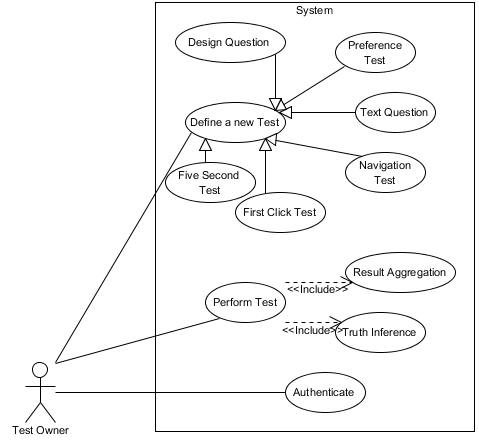
\includegraphics[width=\linewidth]{Resources/usecase_2.PNG}
	\caption[نمودار یوزکیس سامانه هدف]{
		نمودار یوزکیس سامانه هدف
	}
	\label{fig:usecase}
\end{figure}
با توضیحات پیشین، می‌توان نیازمندی‌های مطرح شده پیشین را به مدلی تبدیل کرد که در نمودار یوزکیس موجود در شکل
\ref{fig:usecase}،
قابل مشاهده است.
\section{توضیح کارکرد ابزار}
با کشف نیازمندی‌ها و پیاده‌سازی ابزار، صفحات پیاده‌سازی شده در سامانه کاربردی مبتنی بر وب (ابزار تست نهایی) به شرح زیر پیاده‌سازی شدند که کارکردهای اصلی در تصاویر موجود در شکل
\ref{fig:pages}
قابل مشاهده است.
\begin{figure}
	\centering
	\subfloat[فرم تعریف تست اولین کلیک]{
		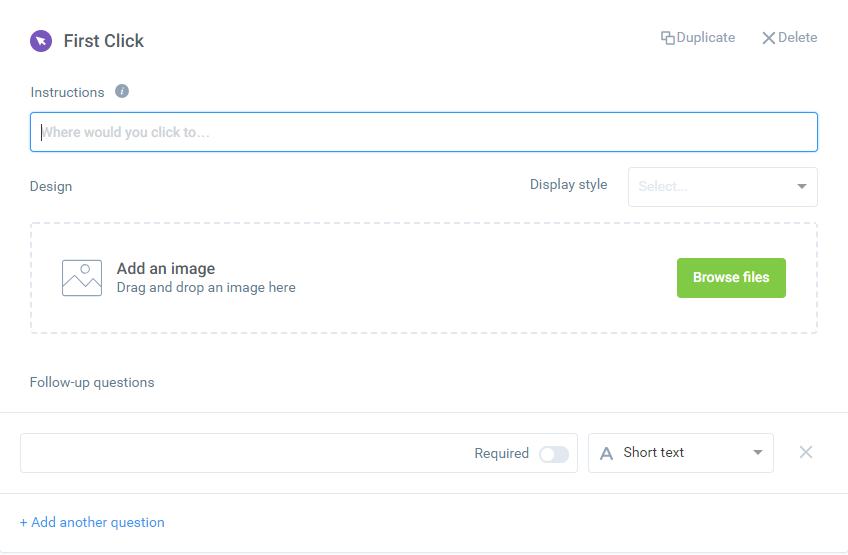
\includegraphics[width=6.5cm]{Resources/tool_1.PNG}
	}
	\subfloat[فرم تعریف تست پنج ثانیه]{
		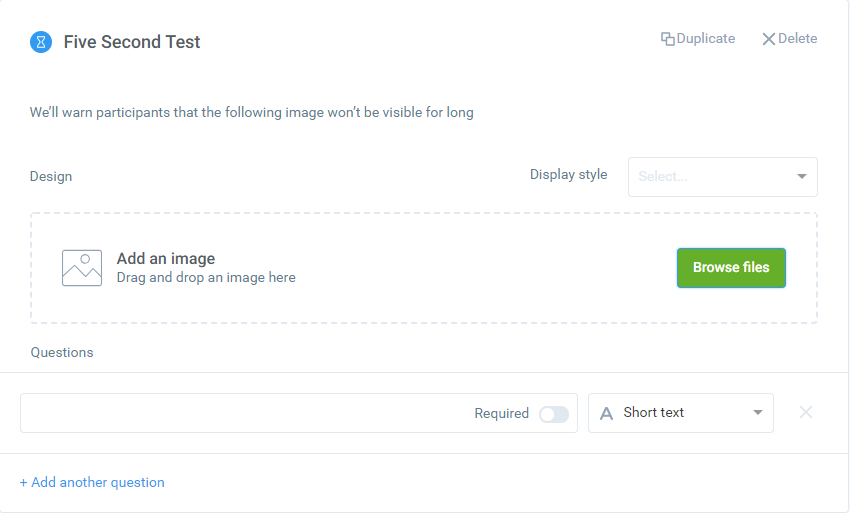
\includegraphics[width=6.5cm]{Resources/tool_2.PNG}
	}
	\hspace{0mm}
	\subfloat[فرم تعریف پرسشنامه متنی]{
		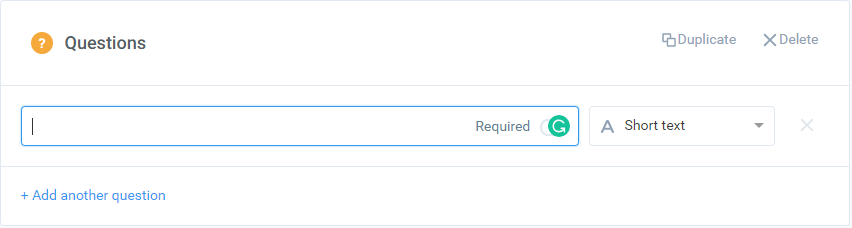
\includegraphics[width=6.5cm]{Resources/tool_3.PNG}
	}
	\subfloat[فرم تعریف پرسشنامه مربوط به طراحی (با عکس)]{
		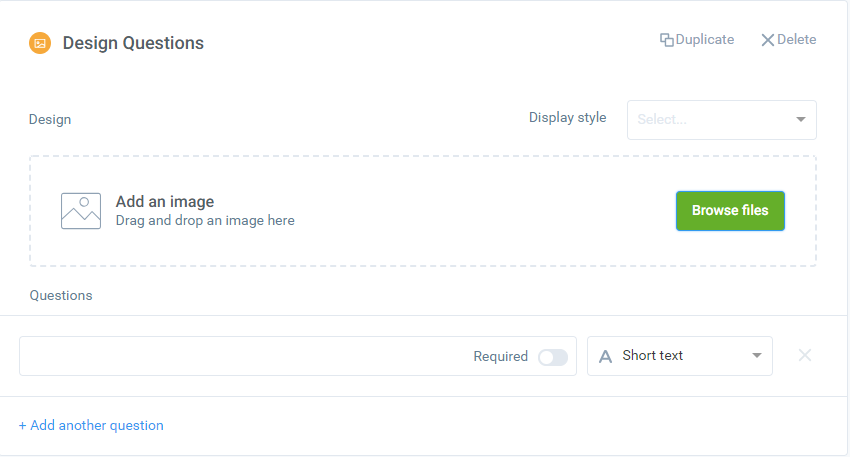
\includegraphics[width=6.5cm]{Resources/tool_4.PNG}
	}
	\hspace{0mm}
	\subfloat[فرم تعریف تست ترجیح]{
		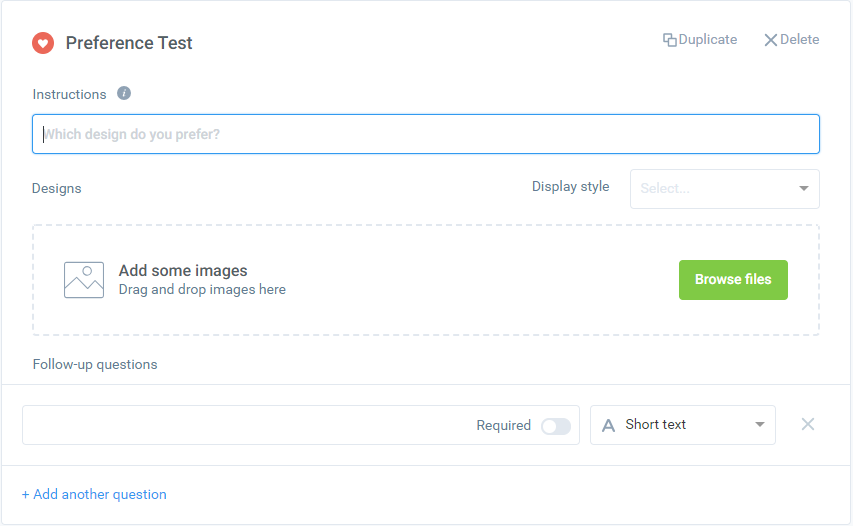
\includegraphics[width=6.5cm]{Resources/tool_5.PNG}
	}
	\subfloat[فرم تعریف تست پیمایش]{
		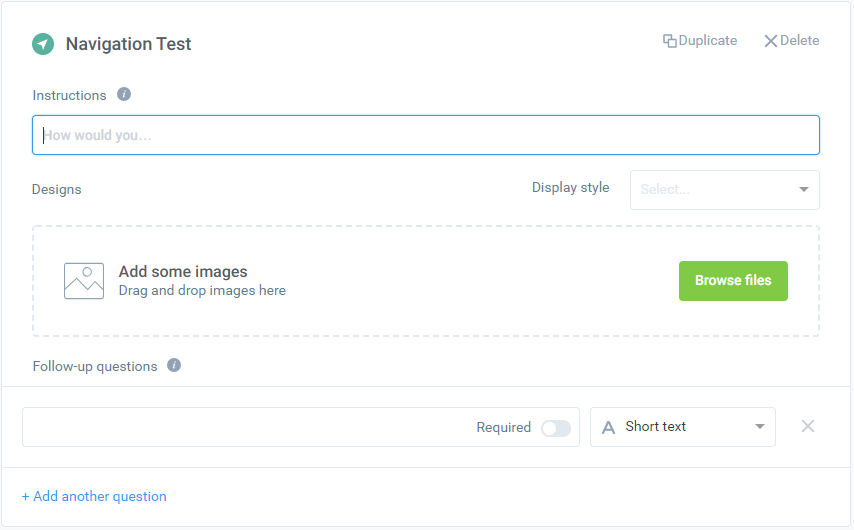
\includegraphics[width=6.5cm]{Resources/tool_6.PNG}
	}
	\caption[فرم‌های تعریف انواع تست‌های مختلف بر اساس الگوهای به دست آمده]
	{فرم‌های تعریف انواع تست‌های مختلف بر اساس الگوهای به دست آمده
	}
	\label{fig:pages}
\end{figure}
کاربران پس از ورود به حساب کاربری خود در سامانه، می‌توانند لیست تست‌های پیشین خود را مشاهده و در صورت لزوم در آن‌ها تغییری ایجاد کنند، حساب خود را مدیریت کنند و یا به ایجاد تست جدید بپردازند. پس از اینکه تست جدید ساخته شد و منتشر گردید، کاربر دارای آدرس وب منحصر به فردی خواهد شد که به طور خاص برای تست مدنظرش است؛ علاوه بر اینکه کاربر می‌تواند با به اشتراک گذاشتن آدرس وب با همگان، آن‌ها را دعوت به شرکت در انجام تست از طریق سامانه بکند، می‌تواند از امکان استفاده از سکوی جمع‌سپاری
\lr{Figure-Eight}\RTLfootnote{
	این سکو، درواقع همان سکوی
	\lr{CrowdFlower} می‌باشد که به تازگی و در سال ۲۰۱۸ تغییر نام داده و به 
	\lr{Figure-Eight}
	تبدیل شده است.
}
که با ابزار مورد نظر با واسط برنامه‌نویسی آن سکو ادغام شده است، بهره ببرد.\\
در هر دو صورت، داده‌های به دست آمده می‌بایست تجمیع شده و درستی و صحت آن‌ها تضمین شود. به منظور تضمین صحت و درستی داده‌ها، از روش تست پنهان استفاده می‌شود؛ همچنین گفتنی است که برای تجمیع داده‌ها و همچنین جلوگیری از تاثیر داده‌های هرز\LTRfootnote{Spam}، از روش کیفیت کارگران بهره گرفته می‌شود
\cite{li_crowdsourced_2016}.


















